\begin{problem}{52/figs/52_pic.jpg}{Non-isomorphic Graphs}  There are $2^{10}$ undirected unweighted graphs with 5 vertices. Two graphs are called isomorphic, if one can obtain one of them by changing the labels of the vertices of the other graph. An example of two isomorphic graphs is given in the figure below.

\begin{center}
	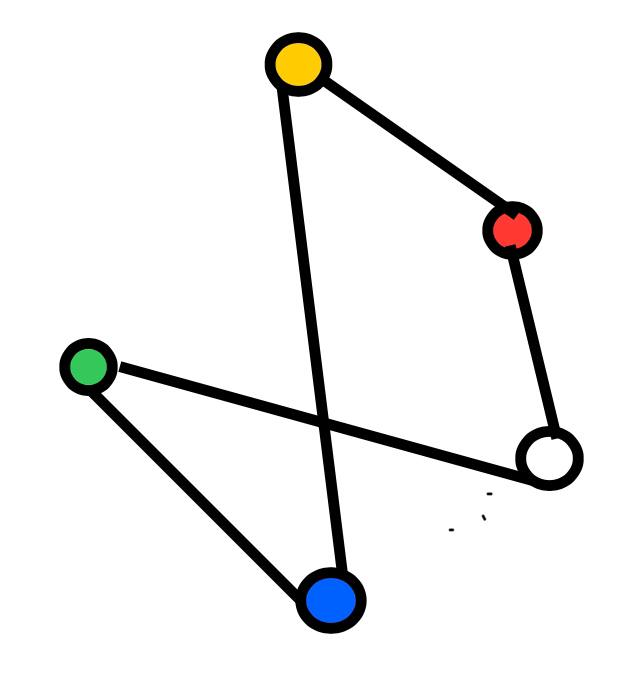
\includegraphics[width=4cm]{52/figs/52_p1.jpg}	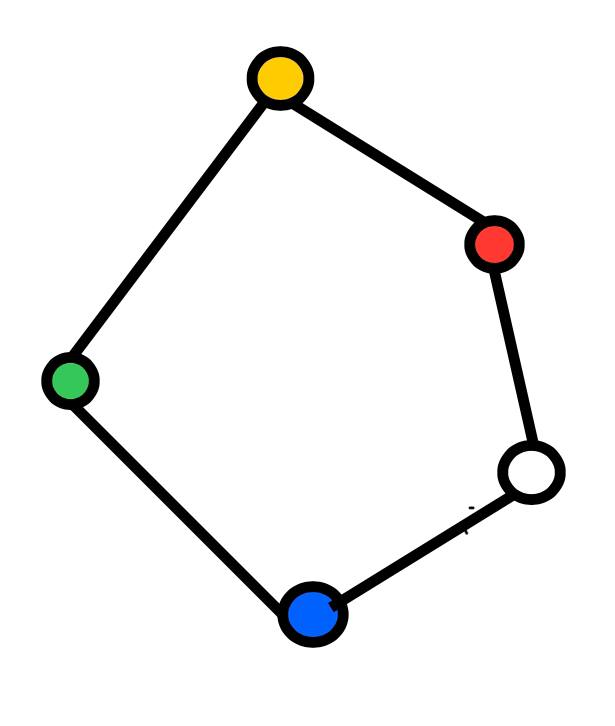
\includegraphics[width=4cm]{52/figs/52_p2.jpg}
\end{center}	

Solve the following problem without using a computer: How many non-isomorphic unweighted undirected graphs with 5 vertices are there?
\end{problem}